\documentclass{article}

\usepackage[fleqn]{amsmath}
\usepackage{amssymb}
\usepackage{hyperref}
\usepackage{url}
\usepackage{graphicx}
\usepackage{geometry}
\usepackage{babel}
\usepackage{enumitem}
\usepackage{parskip}
\usepackage{chemfig}
\usepackage{pdfpages}
\usepackage{xcolor}
\usepackage{tikz}
\usepackage{fancybox}
\usepackage{makecell}
\usepackage{pgfplots}
\usepackage{soul}
\usepackage{ulem}
\usepackage{wrapfig}
\usepackage{subcaption}
\usepackage[T1]{fontenc}
\usepackage{pgfplots}
\usetikzlibrary{arrows}
\usetikzlibrary{decorations.pathreplacing}
\pgfplotsset{compat=1.17}

\geometry{
    a4paper,
    total={170mm, 257mm},
    left=20mm,
    top=20mm
}

\hypersetup{
    colorlinks=true,
    linkcolor=black,
    urlcolor=blue,
    pdftitle={Math refreshing course}
}

\newcommand{\figbox}[1]{ 
    \begin{figure*}[ht!]        
        \begin{center}            
            \fbox{#1}        
        \end{center}    
    \end{figure*}
}

% === TEXT ===
\title{\textbf{Maths refreshing course \\ HSLU, Semester 1}}
\author{Matteo Frongillo}

\begin{document}

\maketitle
\tableofcontents
\pagebreak

\part{Lesson 1}

\section{Algebraic definitions}
\begin{itemize}
    \item $\mathbb{N} := \text{Natural numbers (including 0)}$
    \item $\mathbb{Z} := \text{Integer numbers}$
    \item $\mathbb{Q} := \text{Rational numbers}$
    \item $\mathbb{R} := \text{Real numbers}$
\end{itemize}

\underline{Notation}: The ``$^*$'' symbol means that the set does not include 0.

We have that: 
\[
    \mathbb{N} \subset  \mathbb{Z} \subset \mathbb{Q} \subset \mathbb{R} \subset \mathbb{C} 
\]

\section{Prime numbers}
A prime number is a natural number greater than 1 that has no positive
divisors other than 1 and itself.
\figbox{$n \in \mathbb{N},\ n \neq \{0, 1\}$}

\section{Positive powers}
Let $a \in \mathbb{R}, n \in \mathbb{R}^*$ and ${a} \subset \mathbb{R}$, then

\figbox{$
    a^{1} := a \quad | \quad
    a^n = \underbrace{a \cdot a \cdot ... \cdot a}_{n \text{ times}}$
}

\subsection{Property 1}
Let $a, b \in \mathbb{R},\ n,m \in \mathbb{N}$, then \\
\figbox{$a^n \cdot a^m = a^{n+m}$}

\subsection{Property 2}
Let $a,b \in \mathbb{R},\ n \in \mathbb{N}$, then \\
\figbox{$(a \cdot b)^n = a^n \cdot b^n$}

\underline{Notation}: The power $a^n$, $a$ is the base and $n$ is the exponent.

\subsection{Property 3}
Let $a \in \mathbb{R},\ m,n \in \mathbb{N}^*$, then \\
\figbox{$(a^n)^m = a^{n \cdot m}$, which is $\neq a^{(n^m)}$}

\newpage
\section{Fractions}
\underline{Notation 1}: $a \cdot b = a \times b = ab$ \quad | \quad $\frac{a}{b} = a \div b = a : b$

\underline{Notation 2}: ``$a$'' is called numerator, ``$b$'' is called denominator.

\underline{Notation 3}: $\frac{a}{b},\ a,b \in \mathbb{R},\ b \neq 0$

\subsection{Property 1}
Let $a, b \in \mathbb{R}^*$ and $c, d \in \mathbb{R}$, then\\
\figbox{\large $\frac{a}{b} \cdot \frac{c}{d} = \frac{a \cdot c}{b \cdot d}$}

\subsection{Property 2}
Let $a, b \in \mathbb{R}^*$ and $c, d \in \mathbb{R}$, then\\
\figbox{\large $\frac{a}{b} \div \frac{c}{d} = \frac{a}{b} \cdot \frac{d}{c}$}

\subsection{Property 3}
Let $a, b \in \mathbb{R}^*$ and $c, d \in \mathbb{R}$, then\\
\figbox{\large $\frac{a}{b} \pm \frac{c}{d} = \frac{a \cdot d \pm c \cdot b}{b \cdot d}$}

\section{Negative powers}
\subsection{Definition}
\figbox{$\forall a \in \mathbb{R}^*$; \; $a^{-1} := \frac{1}{a} $}

\subsection{Property 4}
Let $\forall n \in \mathbb{N},\ \forall a \in \mathbb{R}$, then\\
\figbox{$a^{-n} = \left(\frac{1}{a}\right)^n$}

This property implies that $\forall z \in \mathbb{Z},\ \forall a \in \mathbb{R},\ z \neq 0$\\
We can compute $a^z$

\subsection{Property 5}
Let $\forall a \in \mathbb{R},\ a \neq 0,\ \forall n,m \in \mathbb{Z}$, then\\
\figbox{$\frac{a^n}{a^m} = a^{n-m}$}

\newpage
\underline{Consequences}:
\begin{enumerate}
    \item Properties 1, 2 and 3 also hold for integer exponents:
        \begin{itemize}
            \item $\forall a \in \mathbb{R},\ \forall n,m \in \mathbb{Z} \Rightarrow a^n \cdot a^m = a^{n+m}$
            \item $\forall b \in \mathbb{R},\ (a \cdot b)^n = a^n \cdot b^n$
            \item $(a^n)^m = a^{n \cdot m}$
        \end{itemize}  
    \item $\forall a \in \mathbb{R}^*,\ a^0 = a^{1-1} = \frac{a^1}{a^1} = 1 \Rightarrow a^0 = 1$
\end{enumerate}

\section{Fractions and percentages (and back)}
$\alpha \in \mathbb{R},\ n \% \text{ of } \alpha \Longleftrightarrow \frac{n}{100} \cdot \alpha$

\newpage
\part{Lesson 2}

\section{Symbols}
Let $a,b \in \mathbb{R}$, then
\begin{itemize}[label=--]
    \item $a=b \rightarrow$ equality ;
    \item $a \neq b \rightarrow$ inequality ($a$ is not equal to $b$);
    \item $a<b \rightarrow$ minor (a is strictly less than b);
    \item $a\leq b \rightarrow$ minor or equal ($a$ is less or equal than $b$);
    \item $a>b \rightarrow$ major ($a$ is strictly greater than $b$);
    \item $a\geq b \rightarrow$ major ($a$ is greater or equal than $b$).
\end{itemize}

\underline{Example}: $x \in \mathbb{R},\ x \geq 2 \rightarrow 2 \leq x < \infty$

\section{Brackets}
\begin{align}
    &\left(\phantom{-}\right) \text{Parenthesis (round brackets)}\\
    &\left[\phantom{-}\right] \text{Square brackets}\\
    &\left\{\phantom{-}\right\} \text{Braces}
\end{align}

\section{Latin notations}
\begin{itemize}
    \item e.g. = for example;
    \item i.e. = that is / that implies;
    \item q.e.d. = we finally prove it;
    \item $\Box$ = we finally prove it. 
\end{itemize}

\section{The real line (not completed)}
\begin{center}
    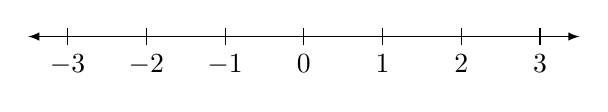
\begin{tikzpicture}
        \draw[latex-latex] (-3.5,0) -- (3.5,0) ; %edit here for the axis
        \foreach \x in  {-3,-2,-1,0,1,2,3} % edit here for the vertical lines
        \draw[shift={(\x,0)},color=black] (0pt,3pt) -- (0pt,-3pt);
        \foreach \x in {-3,-2,-1,0,1,2,3} % edit here for the numbers
        \draw[shift={(\x,0)},color=black] (0pt,0pt) -- (0pt,-3pt) node[below] 
        {$\x$};
    \end{tikzpicture} 
\end{center}  

\subsection{Exercises}
1) \(\forall x \in \mathbb{R}, -3 \leq x \leq 2\)

%\begin{center}
%        \begin{tikzpicture}
%            %number line
%            \draw[-] (-4,0) -- (3,0);
%            \draw[thick] (-3,-0.2) -- (-3,0.2);
%            \draw[thick] (2,-0.2) -- (2,0.2);
%            
%            %interval
%            \draw[thick] (-3,-1) -- (2,-1);
%            \draw[thick] (-3,0) -- (-3,-1);
%            \draw[thick] (2,0) -- (2,-1);
%            \filldraw[black] (-3,-1) circle (2pt);
%            \filldraw[black] (2,-1) circle (2pt);
%            
%            %points
%            \node[above] at (-3,0.2) {-3};
%            \node[above] at (2,0.2) {2};
%            
%            %arrow
%            \draw[->] (3,0) -- (3.5,0);
%
%            %area
%            \draw [draw=black] (-3,0) rectangle (2,-1);
%            \filldraw [fill=Peach, draw=black] (-3,0) rectangle (2,-1);
%            \filldraw [fill=RedOrange, draw=black] (-3,0) rectangle (2,-1);
%        \end{tikzpicture}
%\end{center}

2) \(\forall x \in \mathbb{R}, -2 \leq x \leq 1 \quad \text{and} \quad x > \frac{3}{2}\)

\begin{center}
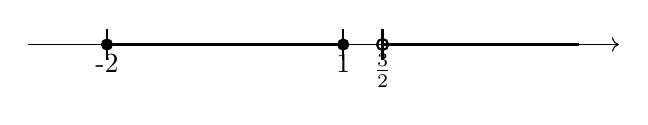
\begin{tikzpicture}
    % Draw the number line
    \draw[-] (-3,0) -- (4,0);
    \draw[thick] (-2,-0.2) -- (-2,0.2);
    \draw[thick] (1,-0.2) -- (1,0.2);
    \draw[thick] (1.5,-0.2) -- (1.5,0.2);
    
    % Draw the intervals
    \draw[thick] (-2,0) -- (1,0);
    \filldraw[black] (-2,0) circle (2pt);
    \filldraw[black] (1,0) circle (2pt);
    \draw[thick] (1.5,0) -- (4,0);
    \draw[thick] (1.5,0) circle (2pt);
    
    % Label the points
    \node[below] at (-2,0) {-2};
    \node[below] at (1,0) {1};
    \node[below] at (1.5,0) {\(\frac{3}{2}\)};
    
    % Draw the arrow
    \draw[->] (4,0) -- (4.5,0);
\end{tikzpicture}
\end{center}

\newpage
\section{Properties of real numbers}
\subsection{Property 1 - Closure of ``$+$'' and ``$\cdot$''}
$\forall x,y \in \mathbb{R}\\
x+y \in \mathbb{R}\\
x \cdot y \in \mathbb{R}$

\underline{Remark}: for $\mathbb{Z}$ this property does not work.

\subsection{Property 2 - Commutativity}
$\forall x,y \in \mathbb{R}\\
x+y=y+x\\
x \cdot y=y \cdot x$

\underline{Remark}: commutativity does not hold for divisions and
subtractions.

\subsection{Property 3 - Associative}
$\forall x,y,z \in \mathbb{R}\\
x+(y+z) = (x+y)+z\\
x \cdot (y\cdot z)=(x\cdot y)\cdot z$

\underline{Remark}: associativity does not hold for divisions and
subtractions.

\subsection{Property 4 - Distributive}
$\forall x,y,z \in \mathbb{R}\\
x(y \pm z)=xy \pm xz$

\subsection{Property 5 - Identity}
$\forall x \in \mathbb{R}$
\begin{enumerate}[label=\alph*)]
    \item $0+x=x$
    \item $1 \cdot x=x$
\end{enumerate}

\underline{Remark}: $\forall x \in \mathbb{R},\ x \cdot 0=0$ is
NOT an identity property.

\subsection{Property 6 - Inverses and opposites}
$\forall x \in \mathbb{R}$
\begin{enumerate}[label=\alph*)]
    \item $x+(-x)=0$ (inverse)
    \item when $x \neq 0,\ x \cdot \frac{1}{x}=1$ (opposite)
\end{enumerate}

\underline{Remark 1}: $\forall x \in \mathbb{N}$ does not exist either
inverse nor opposite.

\underline{Remark 2}: $\forall x \in \mathbb{Z}$ has inverses, but
not opposites.

\section{The order of operations}
\begin{enumerate}
    \item Perform all operations inside grouping symbols beginning with the innermost set:\\
        $\left(\phantom{-}\right)$ inside brackets operations;
    \item Perform all exponential operations as you come to them, moving left-to-right:\\
        $x^a$;
    \item Perform all multiplications and divisions as you come to them, moving left-to-right:\\
        ``$\cdot$'' and ``$\div$'';
    \item Perform all additions and subtractions as you come to them, moving left-by-right:\\
        ``$+$'' and ``$-$'';
    \item When the level of priority is the same (e.g. multiplications and divisions) solve them as you come to them.
\end{enumerate}

\section{Signed numbers}
A number is denoted as positive if it is directly preceded by a $+$ sign or no sign at all.\\
A number is denoted as negative if it is directly preceded by a $-$ sign.

$\forall x \in \mathbb{R}$
\[-(-x)=x\\
+(-x)=-x\\
+(+x)=x\\
-(+x)=-x\]









\end{document}
